
% -*- Mode:TeX -*-

\documentclass[twoside,12pt]{article}
\usepackage{fancyhdr}
\usepackage[margin=1in]{geometry}
\usepackage{hyperref}
\usepackage{enumerate}
\usepackage{enumitem}
\usepackage{graphicx}
\usepackage[nottoc,notlot,notlof]{tocbibind}
\usepackage{amsmath}
\usepackage{listings}
\usepackage{color}
\usepackage[T1]{fontenc}
\usepackage{float}
\usepackage{subcaption}
\usepackage[utf8]{inputenc}
\usepackage{amsfonts}
\usepackage{breqn}
\usepackage{titling}


\author{Andy Wang}

\title{Smooth Shape Interpolation with Multiple Keyframes \\
	\large 6.UAR SuperUROP Proposal \\
	Faculty Advisor: Justin Solomon}

\numberwithin{equation}{section}

\geometry{
  headheight = 3ex,       % <-- and this
	 headsep = 2ex,          % <-- and this
}
\pagestyle{fancy}

\lstdefinestyle{fortranStyle}{
	language=[90]Fortran,
	keywordstyle=\color{red},
	commentstyle=\color{green},
	morecomment=[l]{!\ },
	numbersep=10pt,
	tabsize=4,
	showspaces=false,
	showstringspaces=false,
	basicstyle=\ttfamily\small
}

\newtheorem{lemma}{Lemma}


\begin{document}
\maketitle

\input{TexSections/Abstract}

\section{Introduction}

\section{Previous Work}

\section{Mathematical Background}

\subsection{The Complex Derivatives}

We observe the complex function $f: \Omega \rightarrow \mathbb{R}^2$. This function can also be represented as $f(x,y) = u(x,y) + i v(x,y)$ where $u,v$ are real functions. Using a different notation, $f$ can be written as $f = (u,v)$.

We deal very often with the 2x2 Jacobian of our function $f: \Omega \rightarrow \mathbb{R}^2$. In particular, we desire to decompose the Jacobian into two matrices: the similarity and anti-similarity matrices. Note that this decomposition is also called the "additive decomposition." 

They are defined as:

$$S_2 = \begin{bmatrix}
a & -b \\
b & a
\end{bmatrix}$$

$$A_2 = \begin{bmatrix}
c & d \\
d & -c
\end{bmatrix}$$

Suppose that the Jacobian is the 2x2 matrix 

$$J_f = \begin{bmatrix}
\dfrac{\partial u}{\partial x} & \dfrac{\partial u}{\partial y} \\
\dfrac{\partial v}{\partial x} & \dfrac{\partial v}{\partial y}
\end{bmatrix}
= \begin{bmatrix}
p & q \\ 
r & s
\end{bmatrix}$$

Then we have the decomposition $J_f = S_2 + A_2$ where 
$$\begin{cases}
a = \frac{p+s}{2} \\
b = \frac{r-q}{2} \\
c = \frac{p-s}{2} \\
d = \frac{r+q}{2}
\end{cases}$$


What are these matrices intuitively though? The similarity matrices $S_2$ apply a similarity transformation by rotating and scaling $\mathbb{R}^2$. We can see this by recalling the definition of a 2x2 rotation matrix by angle $\theta$:

$$R_{\theta} = \begin{bmatrix}
\cos \theta & -\sin \theta \\
\sin \theta & \cos \theta 
\end{bmatrix}$$

The similarity matrix is thus the matrix $M R_{\theta}$ where $M = \sqrt{a^2 + b^2}$ and $\theta = \tan^{-1}\left( \frac{b}{a} \right)$. So we can see, that a multiplication of a coordinate vector by similarity matrix $S_2$ corresponds to a rotation by $\theta$ and a scaling by $M$. 

On the other hand, the anti-similarity matrix is simply an application of the same rotation and scaling after a reflection about the x-axis is applied. As we can see:

$$A_2 = M' R_{\theta'} F_y$$
$$= \sqrt{c^2 + d^2} \begin{bmatrix}
\cos \theta' & -\sin \theta' \\
\sin \theta' & \cos \theta' 
\end{bmatrix} \begin{bmatrix}
1 & 0 \\ 
0 & -1
\end{bmatrix}$$ 

where $M' = \sqrt{c^2 + d^2}$ and $\theta' = \tan^{-1} \left(\frac{d}{c}\right)$. 


Now we note that multiplying a vector $z = [x y]^T$ by the similarity matrix $S_2$ is equivalent to multiplying the complex number $(x + iy)$ by $a + ib$. Let us quickly confirm.

$$\begin{bmatrix}a & -b \\ b & a \end{bmatrix} \begin{bmatrix} x \\ y \end{bmatrix} = \begin{bmatrix} xa-by \\ xb + ay \end{bmatrix}$$

$$(a+ib)(x+iy) = (xa-by) + i(xb+ay)$$

Analogously, multiplication by the anti-similarity matrix $A_2$ is equivalent to multiplying $\bar{z} = x-iy$ by $c+id$. This can be confirmed in the same fashion.

Now we come into the definitions of $f_z, f_{\bar{z}}$. These are also called the Wirtinger derivatives $\frac{\partial f}{\partial z}, \frac{\partial f}{\partial \bar{z}}$ respectively. The intuition is that we are effectively computing a change of variable from $(x,y)$ to $(z,\bar{z})$. Let us use the chain rule to determine $\frac{\partial}{\partial z}, \frac{\partial}{\partial \bar{z}}$. 

Since $z = x + iy$, we have that:

$$\begin{cases}
\dfrac{\partial}{\partial x} = \dfrac{\partial}{\partial z} \dfrac{\partial z}{\partial x} + \dfrac{\partial}{\partial \bar{z}} \dfrac{\partial \bar{z}}{\partial x} = \dfrac{\partial}{\partial z} + \dfrac{\partial}{\partial \bar{z}} \\

\dfrac{\partial}{\partial y} = \dfrac{\partial }{\partial z} \dfrac{\partial z}{\partial y} + \dfrac{\partial}{\partial \bar{z}} \dfrac{\partial \bar{z}}{\partial y} = i \dfrac{\partial}{\partial z} - i \dfrac{\partial}{\partial \bar{z}}
\end{cases}$$

This gives us a linear system, which we can solve in order to get that

$$\begin{cases}
\dfrac{\partial}{\partial z} = \dfrac{1}{2} \left( \dfrac{\partial}{\partial x} - i \dfrac{\partial}{\partial y} \right) \\

\dfrac{\partial}{\partial \bar{z}} = \dfrac{1}{2} \left( \dfrac{\partial}{\partial x} + i \dfrac{\partial}{\partial y} \right)
\end{cases}$$

These are our definitions of the Wirtinger derivatives.

Now as it turns out, $f_z = a + ib, f_{\bar{z}} = c + id$ where $a,b,c,d$ are the elements of the matrices in the additive decomposition of the Jacobian of $f$. In order to show this for $f_z$, recall that 

$$f_z = \frac{1}{2} \left( f_x - i f_y \right)$$
$$ = \frac{1}{2} \left( (u_x + i v_x) - i (u_y + i v_y) \right)$$
$$ = \frac{1}{2} \left( (u_x + v_y) + i ( - u_y + v_x ) \right) $$
$$ = a + ib$$

And $f_{\bar{z}} = c + id$ follows by a similar argument.


\subsection{Holomorphic \& Anti-Holomorphic Mappings}

Now we cover holomorphic and anti-holomorphic mappings, which are essential to the study of complex analysis. By definition, holomorphic functions are complex functions $f$ such that $f_{\bar{z}} = 0$. Recall that we can write $f = (u(x,y), v(x,y)) = u(x,y) + i v(x,y)$ where $u,v$ are real functions.

By expanding $f_{\bar{z}}$, we obtain this formula:

$$\frac{1}{2} (f_x + i f_y) = 0$$
$$\frac{\partial u}{\partial x} + i \frac{\partial v}{\partial x} + i \frac{\partial u}{\partial y} - \frac{\partial v}{\partial y} = 0$$
$$\frac{\partial u}{\partial x} + i \frac{\partial v}{\partial x} = \frac{\partial v}{\partial y} - i \frac{\partial u}{\partial y} $$

By matching real parts and imaginary parts, we get

$$\begin{cases}
\dfrac{\partial u}{\partial x} = \dfrac{\partial v}{\partial y} \\
\dfrac{\partial u}{\partial y} = - \dfrac{\partial v}{\partial x}
\end{cases}$$

This system of equations is also called the Cauchy-Riemann equations. Any function that satisfies the Cauchy-Riemann equations also satisfies $f_{\bar{z}} = 0$ and is therefore holomorphic.


Thus, for holomorphic mappings, we know that our jacobian $J_f$, which can be decomposed into similarity and anti-similarity matrices $S_2, A_2$ that are equivalent to $f_z, f_{\bar{z}}$, is a similarity matrix everywhere. The Jacobian would be equivalent to multiplying $\mathbb{C}$ by $f_z$. Note that this value $f_z$ can also be written as $f'$. 

These holomorphic functions are infinitely differentiable. This is not a trivial theorem to prove, and is commonly derived as a corollary of Cauchy's Integral Formula, which states that a holomorphic function defined on a disk is completely determined by its values on the boundary of the disk. In addition, the derivatives and anti-derivatives of holomorphic functions are holomorphic as well. The sums, products, compositions are holomorphic. And the quotients are holomorphic wherever the denominator does not vanish or evaluate to 0.


\subsection{Harmonic Planar Mappings}

Harmonic planar mappings are defined in this section. But first, we begin with harmonic real functions. A real function $u(x,y) : \Omega \rightarrow \mathbb{R}$ is harmonic if it satisfies the Laplace equation

$$\Delta u = \frac{\partial^2 u}{\partial x^2} + \frac{\partial^2 u}{\partial y^2} = 0$$

Harmonic planar mappings are mappings $f : \Omega \rightarrow \mathbb{R}^2$ where $f = (u,v)$ and the $u,v$ are both harmonic real functions. A mapping is simply another name for a function, although in analysis, functions typically are more restrictive and only include mappings from $\mathbb{R}$ to $\mathbb{C}$.

Now, we prove that holomorphic and anti-holomorphic functions are harmonic through the Cauchy Riemann equations. For any holomorphic function $f = (u,v)$, we have that 
$$\Delta u = \frac{\partial^2 u}{\partial x^2} + \frac{\partial^2 u}{\partial y^2}$$
$$ = \frac{\partial}{\partial x} \frac{\partial v}{\partial y} - \frac{\partial}{\partial y} \frac{\partial v}{\partial x}$$
$$ = \frac{\partial^2 v}{\partial x \partial y} - \frac{\partial^2 v}{\partial x \partial y}$$
$$ = 0$$

The argument is similar for $v$. We can then use the same logic to prove that anti-holomorphic functions are also harmonic. 

However, the converse is not necessarily true: Harmonic planar mappings are not necessarily holomorphic nor anti-holomorphic. It is simple to think up an example. % but I won't because I'm too tired.


Now we prove that any harmonic planar mapping $f$ can be written as the sum of a holomorphic function $\phi$ and anti-holomorphic function $\bar{\psi}$:

\begin{equation}
\label{eq:decomposition}
f(z) = \phi(z) + \bar{\psi}(z)
\end{equation}

In order to accomplish this, we bring in harmonic conjugates. Suppose that a real function $u(x,y)$ is harmonic. Then the harmonic conjugate $\hat{v}(x,y)$ is a harmonic real function such that $u + iv$ is holomorphic and thus satisfies the Cauchy-Riemann equations. Look to a complex analysis textbook to see the formula for $\hat{v}$ given $u$. It is not as relevant here. We only need the fact that such a $\hat{v}$ exists.

Since $u$ is harmonic, there exists a harmonic conjugate $\hat{v}$ such that $u + i \hat{v}$ that satisfies the Cauchy-Riemann equations. Since $v$ is harmonic, there exists a harmonic conjugate $\hat{u}$ such that $\hat{u} + i v$ that satisfies the Cauchy-Riemann equations.

If we let $\phi = \frac{u + \hat{u}}{2} + i \frac{v + \hat{v}}{2}$ and $\bar{\psi} = \frac{u - \hat{u}}{2} + i \frac{v - \hat{v}}{2}$, then we can confirm that $\phi$ is holomorphic and $\bar{\psi}$ is anti-holomorphic. In addition $f = \phi + \psi$. 

It also goes that $f_z = \phi'$ and $f_{\bar{z}} = \bar{\psi}'$. We can find this by taking the derivative of Equation \ref{eq:decomposition} with respect to $z, \bar{z}$ and recalling that $f_{\bar{z}} = 0$ for holomorphic functions and $f_{z} = 0$ for anti-holomorphic functions.

Also, intuitively, the parts of the additive decomposition of $J_f$ can be integrated separately to obtain $\phi, \bar{\psi}$. Note that because these functions are integrable because they are holomorphic. 

\subsection{Local Geometric Quantities}

Now we show that some important quantities are representable in terms of the Wirtinger derivatives. First we wish to prove that

$$\det(J_f) = |f_z|^2 - |f_{\bar{z}}|^2$$

Let us approach from the right side:
$$|f_z|^2 - |f_{\bar{z}}|^2 = \frac{1}{4}\left((a^2 + b^2) - (c^2 + d^2)\right)$$
$$ = \frac{1}{4} \left( (p+s)^2 + (r-q)^2 - (p-s)^2 - (r+q)^2 \right) $$
$$ = \frac{1}{4} \left(4ps - 4rq\right) $$
$$ = ps - rq$$
$$ = \det(J_f)$$

and we are done.


Now, a mapping $f$ is locally injective and sense-preserving at point $z$ if $\det(J_f) > 0$. What does it mean to be locally injective? What does it mean to be sense-preserving?
% WHY THOUGH? Give a proof and intuition.

Therefore, $f$ is locally injective and sense-preserving whenever 
$$\det(J_f) = ps - rq > 0$$
$$ps > rq$$
$$(p+s)^2 + (r-q)^2 > (p-s)^2 + (r+q)^2$$
$$a^2 + b^2 > c^2 + d^2$$
$$|f_z|^2 > |f_{\bar{z}}|^2$$
$$|f_z| > |f_{\bar{z}}|$$


Since we desire our mapping $f$ to be locally injective and sense-preserving as part of our desire to produce natural looking animations, we look only at mappings $f$ that satisfy this inequality everywhere. 

Since $|f_{\bar{z}}| \geq 0$, we have that $|f_z| > 0$. 

In the special case of a holomorphic function $g$, recall that $g_{\bar{z}} = 0$ at every point, thus $g' \neq 0$ everywhere and $g$ is a conformal mapping. In other words, it preserves the angle between any two intersection curves. % TODO Why though?
% TODO Is the definition of a conformal mapping such that g' \neq 0 everywhere?

The aim of the paper is to control the amount of conformal (or angular) and isometric (or metric / distance) distortion induced by a mapping. Where we introduce a rigorous definition of these distortion values using singular values of the Jacobian $J_f: 0 \leq \sigma_b \leq \sigma_a$. 

If you look at this \href{http://math.stackexchange.com/questions/861674/decompose-a-2d-arbitrary-transform-into-only-scaling-and-rotation}{ARTICLE}, then you can find out how to retrieve a 2x2 matrix's singular value decomposition (SVD). This gives you the formula for the two singular values $\sigma_a, \sigma_b$:

\begin{equation}
\label{eq:singular-values}
\sigma_a = |f_z| + |f_{\bar{z}}|, \qquad \sigma_b = \left||f_z| - |f_{\bar{z}}|\right|
\end{equation} 

In our case though, we consider mappings that are locally injective and sense-preserving that have $|f_z| > |f_{\bar{z}}|$ so that we can drop the external absolute value sign in $\sigma_b$ to get $\sigma_b = |f_z| - |f_{\bar{z}}| > 0$.

Now we define the first complex dilation as 

$$\mu = \dfrac{f_{\bar{z}}}{f_z}$$

We also define the little dilation as $|\mu|$ or the modulus of the first complex dilation:

$$k = \dfrac{|f_{\bar{z}}|}{|f_z|}$$

This is what we will use to quantify the amount of conformal distortion. % TODO Give intuition as to why this measures conformal distortion.

Observe that our requirement $|f_z| > |f_{\bar{z}}|$ implies that $k = \dfrac{|f_{\bar{z}}|}{|f_z|} < 1$ so that $0 \leq k < 1$ throughout the domain and $k = 0$ when $f_{\bar{z}} = 0$ or $f$ is holomorphic and therefore conformal.















\section{Interpolation Problem}

\section{Parallel Methods}

\section{Metric Pullback}

Another method of interpolating $f_z$ is considered here. In the previous section, we considered interpolating $f_z$ logarithmically. Now, we consider linearly interpolating the metric tensor of $f_z$. 

This method seems to perform the best qualitatively out of the 3 variants presented.

\subsection{The Metric Tensor and Linear Interpolation}

Here, we define the metric tensor. If we consider a planar mapping $h: \Omega \rightarrow \mathbb{R}^2$, then we get that the metric tensor is the matrix expression / version of the pullback metric $h*g$. It is also written as:

\begin{align*}
M_h &= J_h^T J_h \\
&= \begin{bmatrix}|h_z|^2 + |h_{\overline{z}}|^2 & 0 \\ 0 & |h_z|^2 + |h_{\overline{z}}|^2 \end{bmatrix} + 2 \begin{bmatrix}\Re(\eta) & \Im(\eta) \\ \Im(\eta) & -\Re(\eta) \end{bmatrix}
\end{align*}
% you should do this calculation by yourself later


Notice that $M_h$ is symmetric and positive semi-definite.


We may now write the isometric and conformal distortion measures for the purpose of demonstrating that they are bounded when we perform linear interpolation of the metric tensor.

$$\sigma_a^2 = |h_z|^2 + |h_{\overline{z}}|^2 + 2 |\eta| = \mathcal{A} + |\eta|$$
$$\sigma_b^2 = |h_z|^2 + |h_{\overline{z}}|^2 - 2 |\eta| = \mathcal{A} - |\eta|$$

$$K^2 = \frac{\sigma_a}{\sigma_b} = \frac{\mathcal{A} + 2|\eta|}{\mathcal{A} - 2 |\eta|}$$

While linearly interpolating the metric tensor according to $M_h^t = (1-t)M_h^0 + t M_h^1$, we get that due to uniqueness of the additive decomposition, that $\mathcal{A}$ and $|\eta|$ are linearly interpolated as well. % prove this

This makes it clear that isometric distortion is linearly interpolated.



\subsection{Interpolation on the Boundary}

To quote the text, ``the blending of the metric tensor everywhere may not give us metrics that are realizable as the pullback metric for a planar mapping". 

For that reason, we only interpolate the metric tensor on the boundary to determine $f_z$ on the boundary. Then we may solve a Dirichlet problem to determine a harmonic function $u: \Omega \rightarrow \mathbb{R}$ with value $\ln |f_z^t|$ in the interior. % how DO you solve a dirichlet problem?


\subsection{Variant Validation}
% not necessary, just more bound confirmation
% when we are mostly concerned with application








\section{Implementation}

Although the paper gives a continuous formulation of the problem, in practice we must discretize the representation of the shape. We use a 2D triangular mesh that encompasses the used image. The image is then used as a texture for the mesh. 

In order to provide the so-called "keyframes," which are essentially complex transformations of the vertices in the original mesh to a new set of vertices comprising the new mesh, we use the method by [Chen \& Weber 2015]. We call these "keyframes" deformations of the original mesh. 

\subsection{Creating Deformations}

This method by Chen \& Weber is used to generate deformations of the input mesh so that the resulting mappings are of bounded distortion and harmonic. It is particularly important that these deformations be harmonic (or approximately harmonic, since we are discretizing the mapping). The intuition behind this is that harmonic mappings have low Dirichlet energy, which is a metric for how variable / distorted a function is. % why is harmonicity good? Recall that harmonic mappings have low Dirichlet energy (distortion)

These deformations are, as mentioned before, harmonic complex transformations $f$ of the mesh. So to find the resulting vertices, we simply take $f(v)$ for every complex coordinate vertex $v$ in the mesh. It will however, be convenient to represent this harmonic function $f$ as the sum of a holomorphic and anti-holomorphic function $\phi + \overline{\psi}$ as given in Equation \ref{eq:decomposition}. In turn, it is convenient to represent the holomorphic functions $\phi, \psi$ as Cauchy complex barycentric coordinates. These are, in short, the Cauchy coordinates.


\subsubsection{Cauchy Coordinates}

When speaking about a mesh, we can decompose holomorphic functions into the sum of Cauchy coordinates, or functions related to the vertices in the cage of the mesh.

\begin{figure}[h]
	\centering
	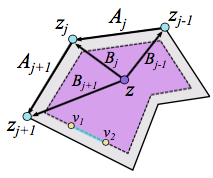
\includegraphics[width=0.25\textwidth]{Images/Cauchy-Cage.png}
	\caption{Cauchy Cage [Chen \& Weber 2015]}
	\label{fig:Cauchy-Cage}
\end{figure}

In this way, any holomorphic function $\Phi(z)$ can be approximated by a linear combination of the finite set of Cauchy barycentric coordinates:

$$\Phi(z) = \sum_{j=1}^n C_j(z) \phi_j$$

where $\phi_j$ is a complex constant.

\subsection{Creating Deformations (Continued)}

We assume the domain's boundary is a simply connected polygon $P$. We can offset the boundary in the outward normal direction to form the cage $\hat{P} = \{z_1, z_2, \ldots, z_n\}, z_i \in \mathbb{C}$. 

$\ldots$

Then after minimizing the ARAP energy in a series of loops, we obtain functions $\Phi, \Psi$ which comprise our mapping $f$. Recall that these functions are written as:

\begin{align} \label{eq:Cauchy-Transform}
\Phi(z) &= \sum_{j=1}^n C_j(z) \phi_j \\
\Psi(z) &= \sum_{j=1}^n C_j(z) \psi_j
\end{align}

where we know the complex numbers $\{\phi_1, \phi_2, \ldots, \phi_n\}, \{\psi_1, \psi_2, \ldots, \psi_n\}$ as well as the closed form representation of TO BE CONTINUED.


\subsection{Integration of $\Phi'$}

In this section, we discuss how to recover $\Phi$ from $f_z = \Phi'$. The difficulty concerning this step arises when considering that the antiderivative of $f_z$, while holomorphic, does not necessarily belong to the subspace of holomorphic functions spanned by Equation \ref{eq:Cauchy-Transform}. 

One such method due to \cite[Chen \& Weber 2015]{bdhm-2015} works by performing a least squares projection of the derivatives into the Cauchy coordinate space.

However, a better approach that %supposedly
produces better results with bounded geometric distortion uses spanning trees to perform an integration of $\Phi'$ to recover $\Phi$. The main idea lies in the rectangle rule:

\begin{equation}
\Phi^t(v_j) - \Phi^t(v_i) = \int_{v_i}^{v_j} f_z^t(z) dz \approx (v_j-v_i) \frac{f_z^t(v_j) + f_z^t(v_i)}{2}
\end{equation}

This lets us calculate the edge differences for all edges in parallel if desired, and then accumulate these values along all the edges of the spanning tree.


Note that we also need one anchor point $\Phi(v_0)$. This point, chosen by the user on the original mesh, may be linearly interpolated according to the equation:

$$\Phi^t(v_0) = (1-t) f^0(v_0) + t f^1(v_0)$$



 


 





\end{document}
